\documentclass[12pt,openright,oneside,a4paper,brazil]{abntex2}
\usepackage[UTF8]{inputenc}
\usepackage{amsmath}
\usepackage{hyperref}
\usepackage[alf]{abntex2cite}
\usepackage[pdftex]{graphicx}
\usepackage{caption}
\usepackage{subcaption}
\usepackage{epstopdf}
\usepackage{multirow}
\usepackage{hhline}
\usepackage[nohyperlinks]{acronym}

%usar centralizar com tamanho fixo de célula
\usepackage{array}
\newcolumntype{L}[1]{>{\raggedright\let\newline\\\arraybackslash\hspace{0pt}}m{#1}}
\newcolumntype{C}[1]{>{\centering\let\newline\\\arraybackslash\hspace{0pt}}m{#1}}
\newcolumntype{R}[1]{>{\raggedleft\let\newline\\\arraybackslash\hspace{0pt}}m{#1}}

\usepackage{hyperref}
\hypersetup{
	pdftitle={\@title},
	pdfauthor={\@author},
	pdfsubject={\imprimirpreambulo},
	pdfkeywords={Sistemas Embarcados}{Segurança}{Tempo Real},
	pdfcreator={Rodrigo Almeida},
	colorlinks=true,
	linkcolor=black,
	citecolor=black,
	urlcolor=black
}

%% pra floats funcionarem melhor
%\renewcommand{\topfraction}{0.50}        % maximo da pagina que pode conter um float (cont de cima
%\renewcommand{\bottomfraction}{0.50}    % maximo da pagina que pode conter um float (cont de baixo
%\setcounter{topnumber}{3}                % maximo de floats no topo
%\setcounter{bottomnumber}{3}            % maximo de floats em baixo
%\setcounter{totalnumber}{5}                % maximo de floats numa unica pagina
%\renewcommand{\textfraction}{0.1}        % minimo de texto em uma pagina
%\renewcommand{\floatpagefraction}{0.5}    % minimo preencido pra fazer uma pagina só de float


%-----------------------------------------------

\usepackage{listings}
\renewcommand{\lstlistlistingname}{Lista de códigos}
\renewcommand{\lstlistingname}{Código}

\makeatletter
\renewcommand*{\numberline}[1]{\hb@xt@2.8em{#1 - \hfil}}
\renewcommand\l@lstlisting[2]{\@dottedtocline{1}{1.5em}{1em}{  Código~#1}{#2}}
\renewcommand\l@figure[2]{\@dottedtocline{1}{1.5em}{1em}{  Figura~#1}{#2}}
\renewcommand\l@table[2]{\@dottedtocline{1}{1.5em}{1em}{  Tabela~#1}{#2}}
\makeatother

\lstset{
	language=C,
	keywordstyle=\bfseries\color[rgb]{0,0,0.627},
	identifierstyle=\ttfamily,
	commentstyle=\itshape\color[rgb]{0.1,0.4,0.1},
	stringstyle=\ttfamily\color[rgb]{0.627,0.126,0.126},
	showstringspaces=false,
	basicstyle=\footnotesize,
	numberstyle=\footnotesize,
	numbers=left,
	stepnumber=1,
	numbersep=6pt,
	tabsize=2,
	breaklines=true,
	prebreak = \raisebox{0ex}[0ex][0ex]{\ensuremath{\hookleftarrow}},
	breakatwhitespace=true,
	aboveskip={1.5\baselineskip},
	columns=fixed,
	upquote=true,
	extendedchars=true,
	numberblanklines=false,
	frame=none,
	inputencoding=latin1,
	numberbychapter=false
}

%--------------------------------------

%why: http://tex.stackexchange.com/questions/784/how-to-change-the-line-spacing-in-my-list-of-figures
% beetwin chapters the LOT and LOF added an space
\newcommand*{\noaddvspace}{\renewcommand*{\addvspace}[1]{}}
\addtocontents{lof}{\protect\noaddvspace}
\addtocontents{lot}{\protect\noaddvspace}


\title{Troca de contexto segura em sistemas operacionais embarcados utilizando de técnicas de detecção e correção de erros}
\author{Rodrigo Maximiano Antunes de Almeida}
\local{Brasil}
\data{\today}
\orientador {Luis Henrique de Carvalho Ferreira}
\coorientador {Carlos Henrique Valério de Moraes}
\instituicao{
Universidade Federal de Itajubá -- UNIFEI
\par
Programa de Pós-Graduação em Engenharia Elétrica}
\tipotrabalho{Tese de doutorado}
\preambulo{Tese apresentada ao Curso de Doutorado em Engenharia Elétrica com ênfase em Automação e Sistemas Elétricos da Universidade Federal de Itajubá como requisito parcial para a defesa de doutorado}


\begin{document}
\imprimircapa
\imprimirfolhaderosto



\begin{agradecimentos}
~

\indent{}Aos meus pais, por todo o apoio e incentivo para meus estudos.

À Ana Paula Siqueira Silva de Almeida, pela compreensão e companheirismo.

Aos meus irmãos, Marcela e Daniel, simplesmente por fazerem parte da minha vida.

Aos professores Luis Henrique de Carvalho Ferreira e Carlos Henrique Valério de Moraes por todo tempo disponibilizado para realização deste trabalho e pelas valiosas orientações.

Ao amigo Enzo pela ajuda na 1ª versão (funcional) do kernel e a amiga Thatyana pelas revisões do documento.

Ao professor Armando pela ajuda nas análises estatísticas e de confiabilidade.

Aos meus alunos de TFG: Adriano, César, Lucas, Henrique e Rafael, pelo auxilio nos \textit{drivers} e nos vários testes.

Ao amigo Alberto Fabiano, que mesmo nas breves conversas sobre segurança e embarcados sempre me trazia novas ideias (\scriptsize{\textit{in memoriam}}\normalsize).

Aos colegas e amigos do grupo de engenharia biomédica pelo apoio, infraestrutura, paciência nas duvidas interessantes e, principalmente, nas não tão interessantes.

A todos aqueles que, direta ou indiretamente, colaboraram para que este trabalho conseguisse atingir os objetivos propostos.
\end{agradecimentos}

\begin{resumo}
A segurança e a confiabilidade em sistemas embarcados são áreas críticas e de recente desenvolvimento. Além das complicações inerentes à área de segurança, existem restrições quanto a capacidade de processamento e de armazenamento destes sistemas. Isto é agravado em sistemas de baixo custo. Neste trabalho, é apresentada uma técnica que, aplicada à troca de contexto em sistemas operacionais, aumentando a segurança destes. A técnica é baseada na detecção e correção de erros em sequência de valores binários. Para realização dos testes, foi desenvolvido um sistema operacional de tempo real e implementado numa placa de desenvolvimento. Observou-se que o consumo de processamento das técnicas de detecção de erro são inferiores às de correção, cerca de 2\% para CRC e 8\% para Hamming. Objetivando-se minimizar o tempo de processamento optou-se por uma abordagem mista entre correção e detecção. Esta abordagem reduz o consumo de processamento medida que os processos que exigem tempo real apresentem uma baixa taxa de execução, quando comparados com o período de troca de contexto. Por fim, fica comprovada a possibilidade de implementação desta técnica em qualquer sistema embarcado, inclusive em processadores de baixo custo.\\
\\
%TODO rever numeros da revisao
	\noindent
	\textbf{Palavras-chaves}: sistemas embarcados, segurança, troca de contexto, correção de erros.
\end{resumo}



\begin{resumo}[Abstract]
Security and reliability in embedded systems are critical areas with recent development. In addition to the inherent complications in the security area, there are restrictions on these systems processing power and storage capacity. This is even worse in low-cost systems. In this work, a technique to increase the system safety is presented. It is applied to the operating systems context switch. The technique is based on the detection and correction of errors in binary sequences. To perform the tests, a real-time operating system was developed and implemented on a development board. It was observed that the use of error detection and error correction techniques are lower than 2\% for CRC and 8\% to Hamming. Aiming to minimize the processing time a mixed approach between correction and detection was selected. This approach reduces the consumption of processing time as the processes that require real-time presents a low execution rate, when compared to the context switch rate. Finally, it is proved to be possible to implement this technique in any embedded system, including low cost processors.\\
\\
%TODO rever numeros da revisao
	\noindent
	\textbf{Key-words}: embedded systems, security, context switch, error correction.
\end{resumo}


\begin{KeepFromToc}
\pdfbookmark[0]{\listtablename}{lof}
\listoffigures
\cleardoublepage

   
%http://tex.stackexchange.com/questions/126654/lstlistoflistings-isnt-showing-the-lstlistingname
\pdfbookmark[0]{\listtablename}{lot}
\listoftables
\cleardoublepage


%os dois comandos abaixo corrigem a fonte do lstlistoflisting
%http://tex.stackexchange.com/questions/27645/customizing-the-list-of-listings-generated-by-lstlistoflistings
\makeatletter
\let\l@lstlisting\l@section
\makeatother 

\let\oldlstlistoflistings\lstlistoflistings
\renewcommand{\lstlistoflistings}{%
  \begingroup%
  \let\oldnumberline\numberline%
  \renewcommand{\numberline}{\lstlistingname~\oldnumberline}%
  \oldlstlistoflistings%
  \endgroup}
  
\pdfbookmark[0]{\listtablename}{lol}
\lstlistoflistings
\cleardoublepage
\end{KeepFromToc}

\chapter*{Lista de Siglas}
\begin{acronym}
\acro{ADC}{ - \textit{Analog to digital converter}}
\acro{CCR}{ - \textit{Condition code register}}
\acro{CI}{ - Circuito integrado}
\acro{CPU}{ - \textit{Central processing unit}}
\acro{CRC}{ - \textit{Cyclic Redundat Check}}
\acro{DAC}{ - \textit{Digital to analog converter}}
\acro{DRAM}{ - \textit{Dynamic random access memory}}
\acro{ECC}{ - \textit{Error-correcting code}}
\acro{EEPROM}{ - \textit{Eletronic erasable programable read only memory}}
\acro{EDF}{ - \textit{Earliest deadline first}}
\acro{FIT}{ - \textit{Failures in time}}
\acro{FPGA}{ - \textit{Field-programmable gate array}}
\acro{MTBF}{ - \textit{Mean time between failures}}
\acro{PC}{ - \textit{Program counter}}
\acro{PID}{ - Proporcional, Integrador, Derivativo}
\acro{RR}{ - \textit{Round robin}}
\acro{RT}{ - \textit{Real time}}
\acro{SO}{ - Sistema operacional}
\acro{SP}{ - \textit{Stack pointer}}
\acro{SPI}{ - \textit{Serial Peripheral Interface}}
\acro{SRAM}{ - \textit{Static random access memory}}
\acro{VHDL}{ - \textit{VHSIC Hardware Description Language}}
\end{acronym}

\newpage

\pdfbookmark[0]{\contentsname}{toc}
\tableofcontents*
\cleardoublepage

\textual
\setcounter{page}{1}
\chapter{Introdução}

A programação para sistemas embarcados exige uma série de cuidados especiais pois estes sistemas geralmente possuem restrições de memória e processamento \citeonline{barrosintroduccao}. Outra complexidade encontrada é a variedade de arquiteturas e modelos de interfaces disponíveis.

Um dos modos de se reduzir esta complexidade é a utilização de um sistema operacional (SO) que insira uma camada de abstração entre o \textit{hardware} e a aplicação. Esta redução, no entanto, vem acompanhada de uma sobrecarga, tanto no uso de memória, quanto no uso do processador. Esta sobrecarga pode ser proibitiva para alguns dispositivos, principalmente os de menor custo. Segundo \cite{aomontagem}


\section{Objetivo}
%TODO rever ainda o objetivo, 
%Desenvolver um sistema operacional com maior segurança para dispositivos embarcados.

Apresentar uma metodologia aplicável em sistemas embarcados de baixo custo que aumente a robustez do sistema reduzindo os problemas advindos de erros em \textit{bits} de memória. Dentre os objetivos específicos temos:

\begin{itemize}
	\item O sistema deve consumir o mínimo de recursos possível para ser aplicável em sistemas de baixo custo.
	\item A técnica não pode prejudicar a capacidade de execução de processos com requisitos de tempo real.
	\item A metodologia deve proteger o sistema contra vulnerabilidades que possam ser exploradas maliciosamente.
\end{itemize}


\section{Organização do documento}

%TODO refazer
Este documento é organizado em seis capítulos. O segundo capítulo apresenta os conceitos e ferramentas necessários para o desenvolvimento do projeto. O terceiro capítulo contém as etapas do desenvolvimento deste projeto, as dificuldades encontradas bem como as soluções propostas. O quarto capítulo contém a metodologia proposta neste trabalho. Os resultados obtidos foram compilados e apresentados no quinto capítulo. O sexto capítulo reúne as conclusões obtidas bem como a continuidade vislumbrada para este trabalho.

\chapter{Revisão Bibliográfica}


\section{Sistemas Operacionais}

O sistema operacional, SO, é um conjunto de códigos que funciona como uma camada de abstração do \textit{hardware} provendo funcionalidades para as aplicações de alto nível \cite{wulf1974hydra}. Este isolamento permite que a aplicação não sofra alteração quando há mudança no \textit{hardware}. Esta é uma característica muito desejada em sistemas embarcados, onde existe uma pluralidade nos tipos de periféricos dificultando a reutilização de código.

De modo geral, os sistemas operacionais possuem três principais responsabilidades \cite{silberschatz2009operating}:

\begin{itemize}
	\item manusear a memória disponível e coordenar o acesso dos processos a ela;
	\item gerenciar e coordenar a execução dos processos através de algum critério;
	\item intermediar a comunicação entre os periféricos de \textit{hardware} e os processos.
\end{itemize}

Estas responsabilidades se relacionam com os três recursos fundamentais de um sistema computacional: o processador, a memória e os dispositivos de entrada e saída. A Figura~\ref{fig:kernel_int} ilustra estes recursos bem como o papel de interface que um sistema operacional deve realizar.

\begin{figure}[htbp]
	\begin{center}
	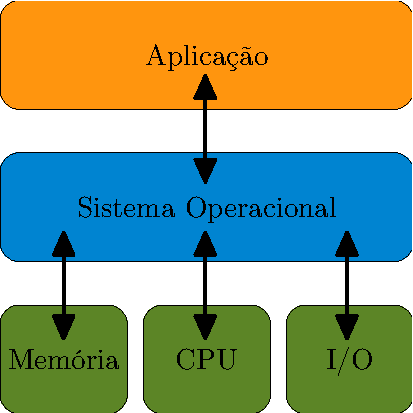
\includegraphics[width=0.6\textwidth]{img/interfaceKernel.pdf}
	\caption{Interfaceamento realizado pelo sistema operacional}
	\label{fig:kernel_int}
	\end{center}
\end{figure}

A ausência de um sistema operacional implica que toda a responsabilidade de organizar o andamento dos processos, os acessos ao \textit{hardware} e o gerenciamento da memória é do programador. Este aumento de responsabilidade, a baixa capacidade de reutilização de código, e a consequente necessidade de recriar os códigos e rotinas, podem ser causadores de erros nos programas.

A capacidade de se reutilizar os programas é benéfica por dois pontos principais: diminui o tempo para entrega do projeto e permite que o programador utilize melhor o tempo, eliminando os erros ao invés de recriar os códigos.


\subsection{Processo}
Na utilização de um sistema operacional, as tarefas a serem executadas pelo processador são organizadas em programas. O programa é uma sequência de comandos ordenados com uma finalidade específica. No momento em que este programa estiver em execução no processador ele passa a ser definido como processo \cite{stallings2009operating}.

Além do código a ser executado, os processos necessitam de posições de memórias extras para armazenar seus dados e variáveis, sejam eles persistentes ou não. São necessárias também regiões de memória, geralmente implementadas em estrutura de pilha, para armazenamento de informações referentes à sequência de execução do programa.

Para realizar o correto gerenciamento dos processos é necessário que o \textit{kernel} possua informações sobre os mesmos, agrupadas de maneira consistente. As informações mínimas necessárias são:

\begin{itemize}
	\item O código a ser executado;
	\item As variáveis internas do processo;
	\item Ponteiros para as informações anteriores, permitindo sua manipulação.
\end{itemize}

Em geral o código fica numa memória não volátil por questões de custo. Para microcontroladores, essas memórias são implementadas em tecnologia EEPROM, ou \textit{flash}. Já as variáveis são armazenadas em memória volátil, pela maior velocidade de acesso e facilidade de escrita. As duas tecnologias mais utilizadas para este tipo de memória são a SRAM e a DRAM.


\subsection{Escalonadores}
Uma das funções principais do \textit{kernel} de um sistema operacional é o gerenciamento dos processos em execução \cite{silberschatz2009operating}. Tal tarefa possui maior importância no contexto de sistemas embarcados, nos quais os processos costumam possuir restrições rígidas quanto ao atraso na execução \cite{barr1999programming}.

Os algoritmos responsáveis por gerenciar e decidir qual dos processos será executado pelo processador são conhecidos como escalonadores. Existem diversas abordagens diferentes para realizar este gerenciamento. Em geral os algoritmos visam a equilibrar o atraso entre o início da execução e a quantidade de processos executados por unidade de tempo. Outros parâmetros importantes para a comparação dos escalonadores são o consumo extra de processamento (\textit{CPU overhead}), a quantidade de processos executados por unidade de tempo (\textit{throughput}), o tempo entre a submissão de um processo e o fim da sua execução (\textit{turnarround time}) e o tempo entre a submissão do processo e a sua primeira resposta válida (\textit{response time}).

Na Tabela~\ref{tab:AlgEscalon} são apresentados quatro algoritmos e as características destes.

\begin{table}[htbp]
	\begin{center}
	\captionof{table}{Algoritmos para escalonamento, vantagens e desvantagens \cite{rao2009simplified}}
	\label{tab:AlgEscalon}
	\begin{tabular}{|m{5cm}|C{2.2cm}|C{2.2cm}|C{2.2cm}|C{2.2cm}|}
		\hline
		Algoritmo de escalonamento & \textit{CPU Overhead} & \textit{Throughput} & \textit{Turnaround time} & \textit{Response time}\\\hline
		Escalonador baseado em prioridade & Baixo & Baixo & Alto & Alto\\\hline
		Escalonador round-robin (RR) & Baixo & Médio & Médio & Alto\\\hline
		\textit{Deadline} mais crítico primeiro (EDF) & Médio & Baixo & Alto & Baixo\\\hline		
		Escalonador de fila multi-nível & Alto & Alto & Médio & Médio\\\hline
	\end{tabular}
	\end{center}
\end{table}

Nota-se pela Tabela~\ref{tab:AlgEscalon} que não existe alternativa ótima, sendo necessário escolher então a que mais se ajusta ao sistema que será desenvolvido.

Para um sistema de tempo real, o tempo de resposta é um dos quesitos mais importantes, dado que a perda de um prazo pode impactar negativamente no funcionamento deste. Algumas aplicações podem falhar se estes requisitos não forem atendidos \cite{reneaux1999}. Apesar disto, nem todos os processos em um sistema embarcado precisam deste nível de determinismo. Deste modo, um escalonador que permita ao programador escolher entre pelo menos dois níveis de prioridade (normal e tempo real) é uma boa alternativa \cite{peek2013complexity}.

A maioria dos sistemas operacionais de tempo real apresentam como opção implementada o escalonador baseado em prioridades. Este fato se deve ao baixo consumo, mas principalmente a capacidade deste sistema de garantir que os processos mais críticos serão sempre executados. Na Tabela~\ref{tab:OSescalonadores} é apresentada a tendência entre vários sistemas operacionais, comerciais e de código aberto. 

Sabendo-se que as falhas acontecem seguindo uma distribuição de poisson \cite{li2006model}, a probabilidade de não ocorrer nenhuma falha ($Pr(0)$), num tempo $\tau$ é dada pela equação~\ref{eq:probFalha}.

\begin{equation}\label{eq:probFalha}
Pr(0) = \frac{e^{-\lambda \tau} (\lambda \tau)^0}{0!} = e^{-\lambda \tau}
\end{equation}

Um parâmetro de confiabilidade muito utilizado \cite{breyfogle2003implementing} quando se espera que não haja defeitos num determinado lote de produtos é o intervalo de quatro sigma e meio, $4,5\sigma$, que representa $3,4$ falhas a cada milhão de unidades. Este intervalo é utilizado para projetos com a metodologia $6\sigma$. Utilizando-se este valor, pode-se considerar que, na prática, não há falhas num processo do tipo $6\sigma$ \cite{geoff2001six}.

Levando-se em conta novamente a distribuição de Poisson é possível calcular qual é o tempo decorrido para que a probabilidade de falha atinja o valor de 0.00034\% ou 3.4 partes por milhão. Considerando-se um alto volume de unidades, este valor também pode ser interpretado como a quantidade esperada de produtos que possuem ou apresentam falhas. Deste modo, é possível calcular o tempo de funcionamento mínimo para que pelo menos 4 unidades, por milhão em funcionamento, apresentem problemas. Este valor, bem mais restritivo que o MTBF, pode ser ponto de comparação entre a qualidade relativa de diferentes produtos ou tecnologias. 



\begin{table}[htbp]
	\begin{center}
	\captionof{table}{Probabilidade de falha em níveis sigma}
	\label{tab:taxasFalhaSigma}
\begin{tabular}{|C{2cm}|C{4cm}|C{8cm}|}
\hline
Intervalo sigma & Quantidade de equipamentos $q$ & Tempo em funcionamento antes que $q$ equipamentos tenham 1 bit errado (Horas)\\ \hline
$1 \sigma$ & 31,752\% & 208.996\\ \hline
$2 \sigma$ & 4,551\% & 25.501\\ \hline
$3 \sigma$ & 0,27\% & 1.480\\ \hline
$4 \sigma$ & 0,007\% & 38\\ \hline
$4,5 \sigma$ & 0,00034\% & 2\\ \hline
\end{tabular} 
	\end{center}
\end{table}


\subsection{Exploração de vulnerabilidades}
Todos os sistemas computacionais estão de algum modo susceptíveis a sofrerem ataques externos. Estes ataques nem sempre visam a invasão do sistema para roubo de informação ou uso não autorizado do mesmo. Alguns ataques podem ter como objetivo apenas desabilitar ou destruir os sistemas alvos.

A técnica de ataque via \textit{buffer overflow} tenta utilizar uma falha na recepção e escrita de um conjunto de dados num \textit{buffer} de memória de tal modo que outras variáveis tenham seu valor alterado. Em processadores de arquitetura Von Neumman, onde o espaço de endereçamento de dados e programas é único, existe a possibilidade de se alterar até mesmo o código do programa armazenado. O programa apresentado no Código~\ref{cod:funOver} possui a possibilidade de explorar um \textit{bug} de \textit{buffer overflow}\cite{wiki2013buffer}.

\begin{lstlisting}[float,caption=Exemplo de função com vulnerabilidade de \textit{buffer overflow},label=cod:funOver]
#include <string.h>
void buffOver (char *bar)
{
   char  c[12];
   strcpy(c, bar);  //sem checagem de tamanho
}
 
int main (int argc, char **argv)
{
   buffOver(argv[1]); 
}
\end{lstlisting}
 
Em geral, os compiladores alocam as variáveis locais na pilha do processo corrente, facilitando o acesso e permitindo que este espaço seja posteriormente desocupado facilmente e liberado para outras aplicações.

Por causa do modo de operação da pilha, as variáveis são alocadas próximas ao endereço de retorno da função chamada, como pode ser observado na Figura~\ref{fig:buffOverAntes}.

Caso seja fornecida uma entrada com menos de 12 caracteres, incluindo o terminador, estes serão armazenados corretamente na pilha sem sobreescrever nenhuma outra variável. A figura \ref{fig:buffOverTeste} apresenta o mapa da memória para a entrada ``Teste''.

\begin{figure}[ht]
        \center
        \begin{subfigure}[b]{0.4\textwidth}
        	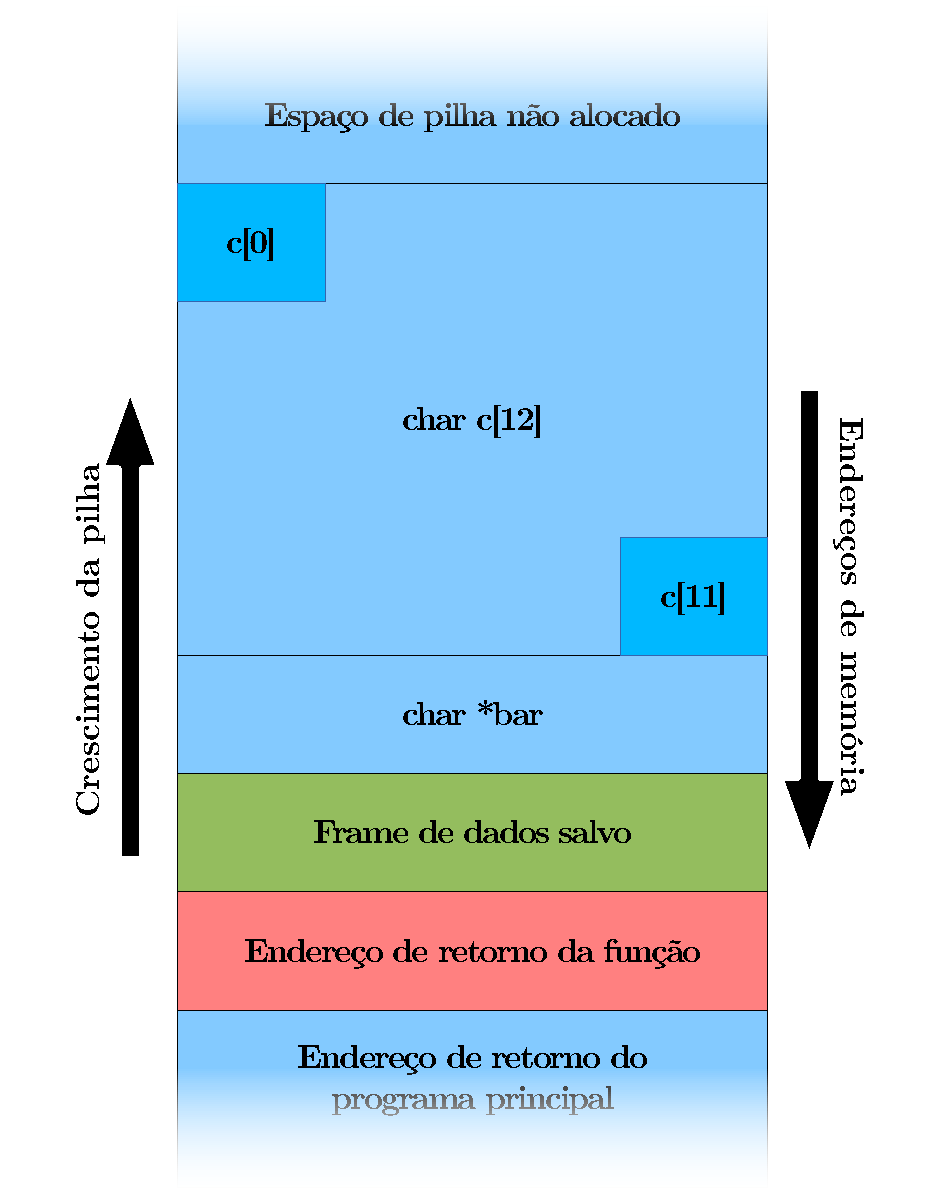
\includegraphics[width=\textwidth]{img/bufferOverAntes.pdf}
        	\caption{Mapa de memória}
        	\label{fig:buffOverAntes}
        \end{subfigure}
        \begin{subfigure}[b]{0.4\textwidth}
        	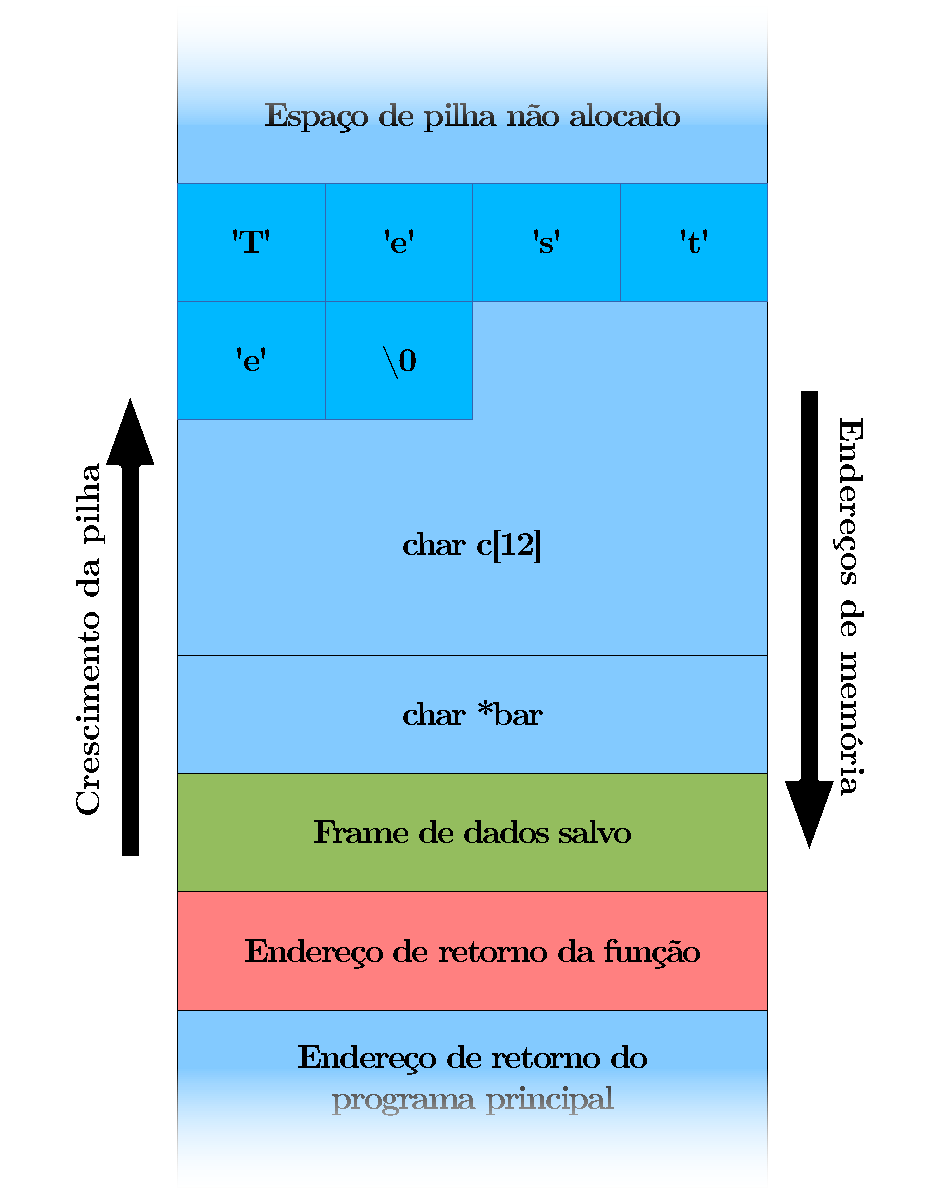
\includegraphics[width=\textwidth]{img/bufferOverTeste.pdf}
        	\caption{Entrada de dados normal}
        	\label{fig:buffOverTeste}
        \end{subfigure}
        \caption{Posicionamento das variáveis e informações na pilha da função \textit{buffOver()}}
\end{figure}

\subsection{CRC}

Os algoritmos de CRC (\textit{Cyclic Redundant Check}) são otimizados para a detecção de erros. Segundo \citeonline{ray2006efficient}, em sistemas com alta exigência na detecção de erros, o algoritmo de CRC pode ser ``a única alternativa prática comprovada pela utilização em campo''.

Estes algoritmos são baseados na divisão inteira de números binários sobre um campo finito de ordem 2. Para efeitos matemáticos de isolação dos coeficientes \cite{williams1993painless}, é comum representar os números como um polinômio de $x$. O termo $x^n$ existe se a posição $n$ da palavra binária for de valor um. Caso o valor seja zero o termo é omitido da representação, conforme exemplo abaixo. %todo ref eq

\begin{equation}
P(x) = x^8 + x^6 + x^0 => 1~0100~0001_2
\end{equation}

Para o cálculo do valor de CRC de uma mensagem representada pelo polinômio $M(x)$ de tamanho $t_m$, dado um polinômio gerador $G(X)$ de tamanho $t_g$, deve-se:
\begin{itemize}
	\item adicionar $t_g$ zeros ao final da mensagem, o que é feito multiplicando o polinômio $M(x)$ por $x^{t_g}$
	\item realizar a divisão deste polinômio $(M(x)\cdot x^{t_g})$ por $G(x)$
	\item armazenar o resto da divisão, o polinômio $R(x)$, em formato binário, que é o valor de CRC
\end{itemize}

Como o resultado do procedimento vem do cálculo do resto de uma divisão, o tamanho do CRC é fixo e determinado pelo termo de maior expoente do polinômio $G(x)$ \cite{kurose2012computer}.

Após a transmissão dos dados, ou na leitura de um valor armazenado a priori, o procedimento de validação dos dados $M'(x)$  é o mesmo para a geração do valor de CRC. Após realizar o cálculo da divisão de $(M'(x)\cdot x^{t_g})$ por $G(x)$, se o valor $R'(x)$, recém calculado, for igual ao valor $R(x)$, armazenado anteriormente, a mensagem foi lida/transmitida corretamente. É possível também realizar a divisão de $M'(x)\cdot x^{t_g} + R(x)$ por $G(x)$ esperando que o resto $R'(x)$ seja igual a 0. 

A escolha do polinômio divisor G(x) é pautada basicamente por dois requerimentos, gasto computacional e quantidade de erros identificáveis dado um determinado tamanho de mensagem. A capacidade de identificar uma dada quantidade de erros binários numa mensagem é denominada distância de Hamming (HD, \textit{hamming distance}). Aplicações críticas geralmente requerem altas distâncias de Hamming, HD = 6 para todos os tamanhos de mensagens \cite{ray2006efficient}.

\citeonline{koopman2004cyclic} apresentam, em seu trabalho, uma tabela com os melhores polinômios com tamanho variando entre 3 e 16 \textit{bits}. Deve-se tomar cuidado na seleção, pois alguns polinômios amplamente utilizados na literatura não apresentam um bom resultado, podendo ser melhorados sem impactar no tempo de cálculo. A Figura~\ref{fig:bestCRC} apresenta os resultados encontrados.

\chapter{Desenvolvimento}

Tradicionalmente, os sistemas de proteção à memória são implementados em \textit{hardware} por questões de velocidade \cite{chaudhari2013framework,lemay2012cumulative}. As soluções em \textit{software}, em geral, apresentam um consumo muito alto \cite{pax2012h2hc,kai2012secure, yim2011hauberk,van2004new}. Uma opção para reduzir esse consumo é realizar a proteção apenas das regiões mais importantes, que normalmente são os objetos do \textit{kernel} \cite{borchert2013generative}. No entanto, estas abordagens são focadas em sistemas \textit{desktops} ou para embarcados com maior capacidade computacional, sendo inviáveis para processadores de baixo custo.

Entre sistemas que utilizam processadores de baixo custo estão diversos controladores industriais, painéis de elevadores comerciais, sensores inteligentes, carros e grande parte de eletrônicos com pouca interação humana.

A Figura~\ref{fig:KernelSeguro} apresenta a solução proposta: realizar a verificação de erros em toda troca de contexto através de informações extras armazenadas na pilha de dados. Todos os acessos realizados pela troca de contexto terão suporte de um sistema de verificação de integridade da informação utilizando os algoritmos de CRC ou Hamming.

\begin{figure}[htbp]
	\begin{center}
	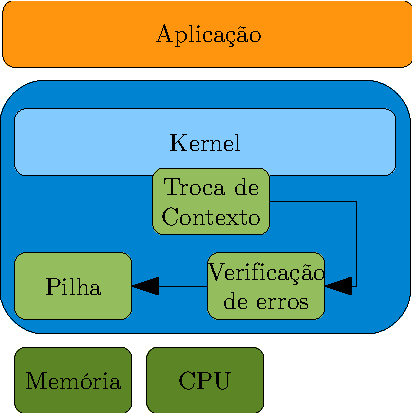
\includegraphics[width=7cm]{img/interfaceKernelSeguro.pdf}
	\caption{Modelo de sistema com verificação de erros na pilha}
	\label{fig:KernelSeguro}
	\end{center}
\end{figure}

Optou-se neste trabalho por realizar a proteção por meio de algoritmos que gerem um código de verificação por bloco de memória, evitando-se assim o gasto demasiado de memória RAM. Com relação ao consumo de processamento foi dada preferência para os algoritmos mais simples com capacidade de correção ou detecção de erros.

%TODO reescrever pensando no método mix do escalonador
As rotinas de troca de contexto de um sistema operacional são bastante complexas, primeiro por serem muito particulares para cada processador e segundo por possuírem códigos em \textit{assembly}, de difícil adaptação.

Por este motivo optou-se pela utilização de um sistema operacional desenvolvido pelos autores \cite{de2013microkernel}, facilitando a adaptação das rotinas necessárias na troca de contexto. O sistema operacional foi separado em 4 camadas: aplicação (amarelo), microkernel (vermelho), controladora de drivers (azul) e os drivers (preto e verde). A Figura~\ref{fig:diagramaClasse} apresenta um resumo do sistema desenvolvido, a interligação do \textit{kernel} com a aplicação e a controladora de \textit{drivers} bem como todos os \textit{drivers} implementados.

\begin{figure}[htbp]
	\begin{center}
	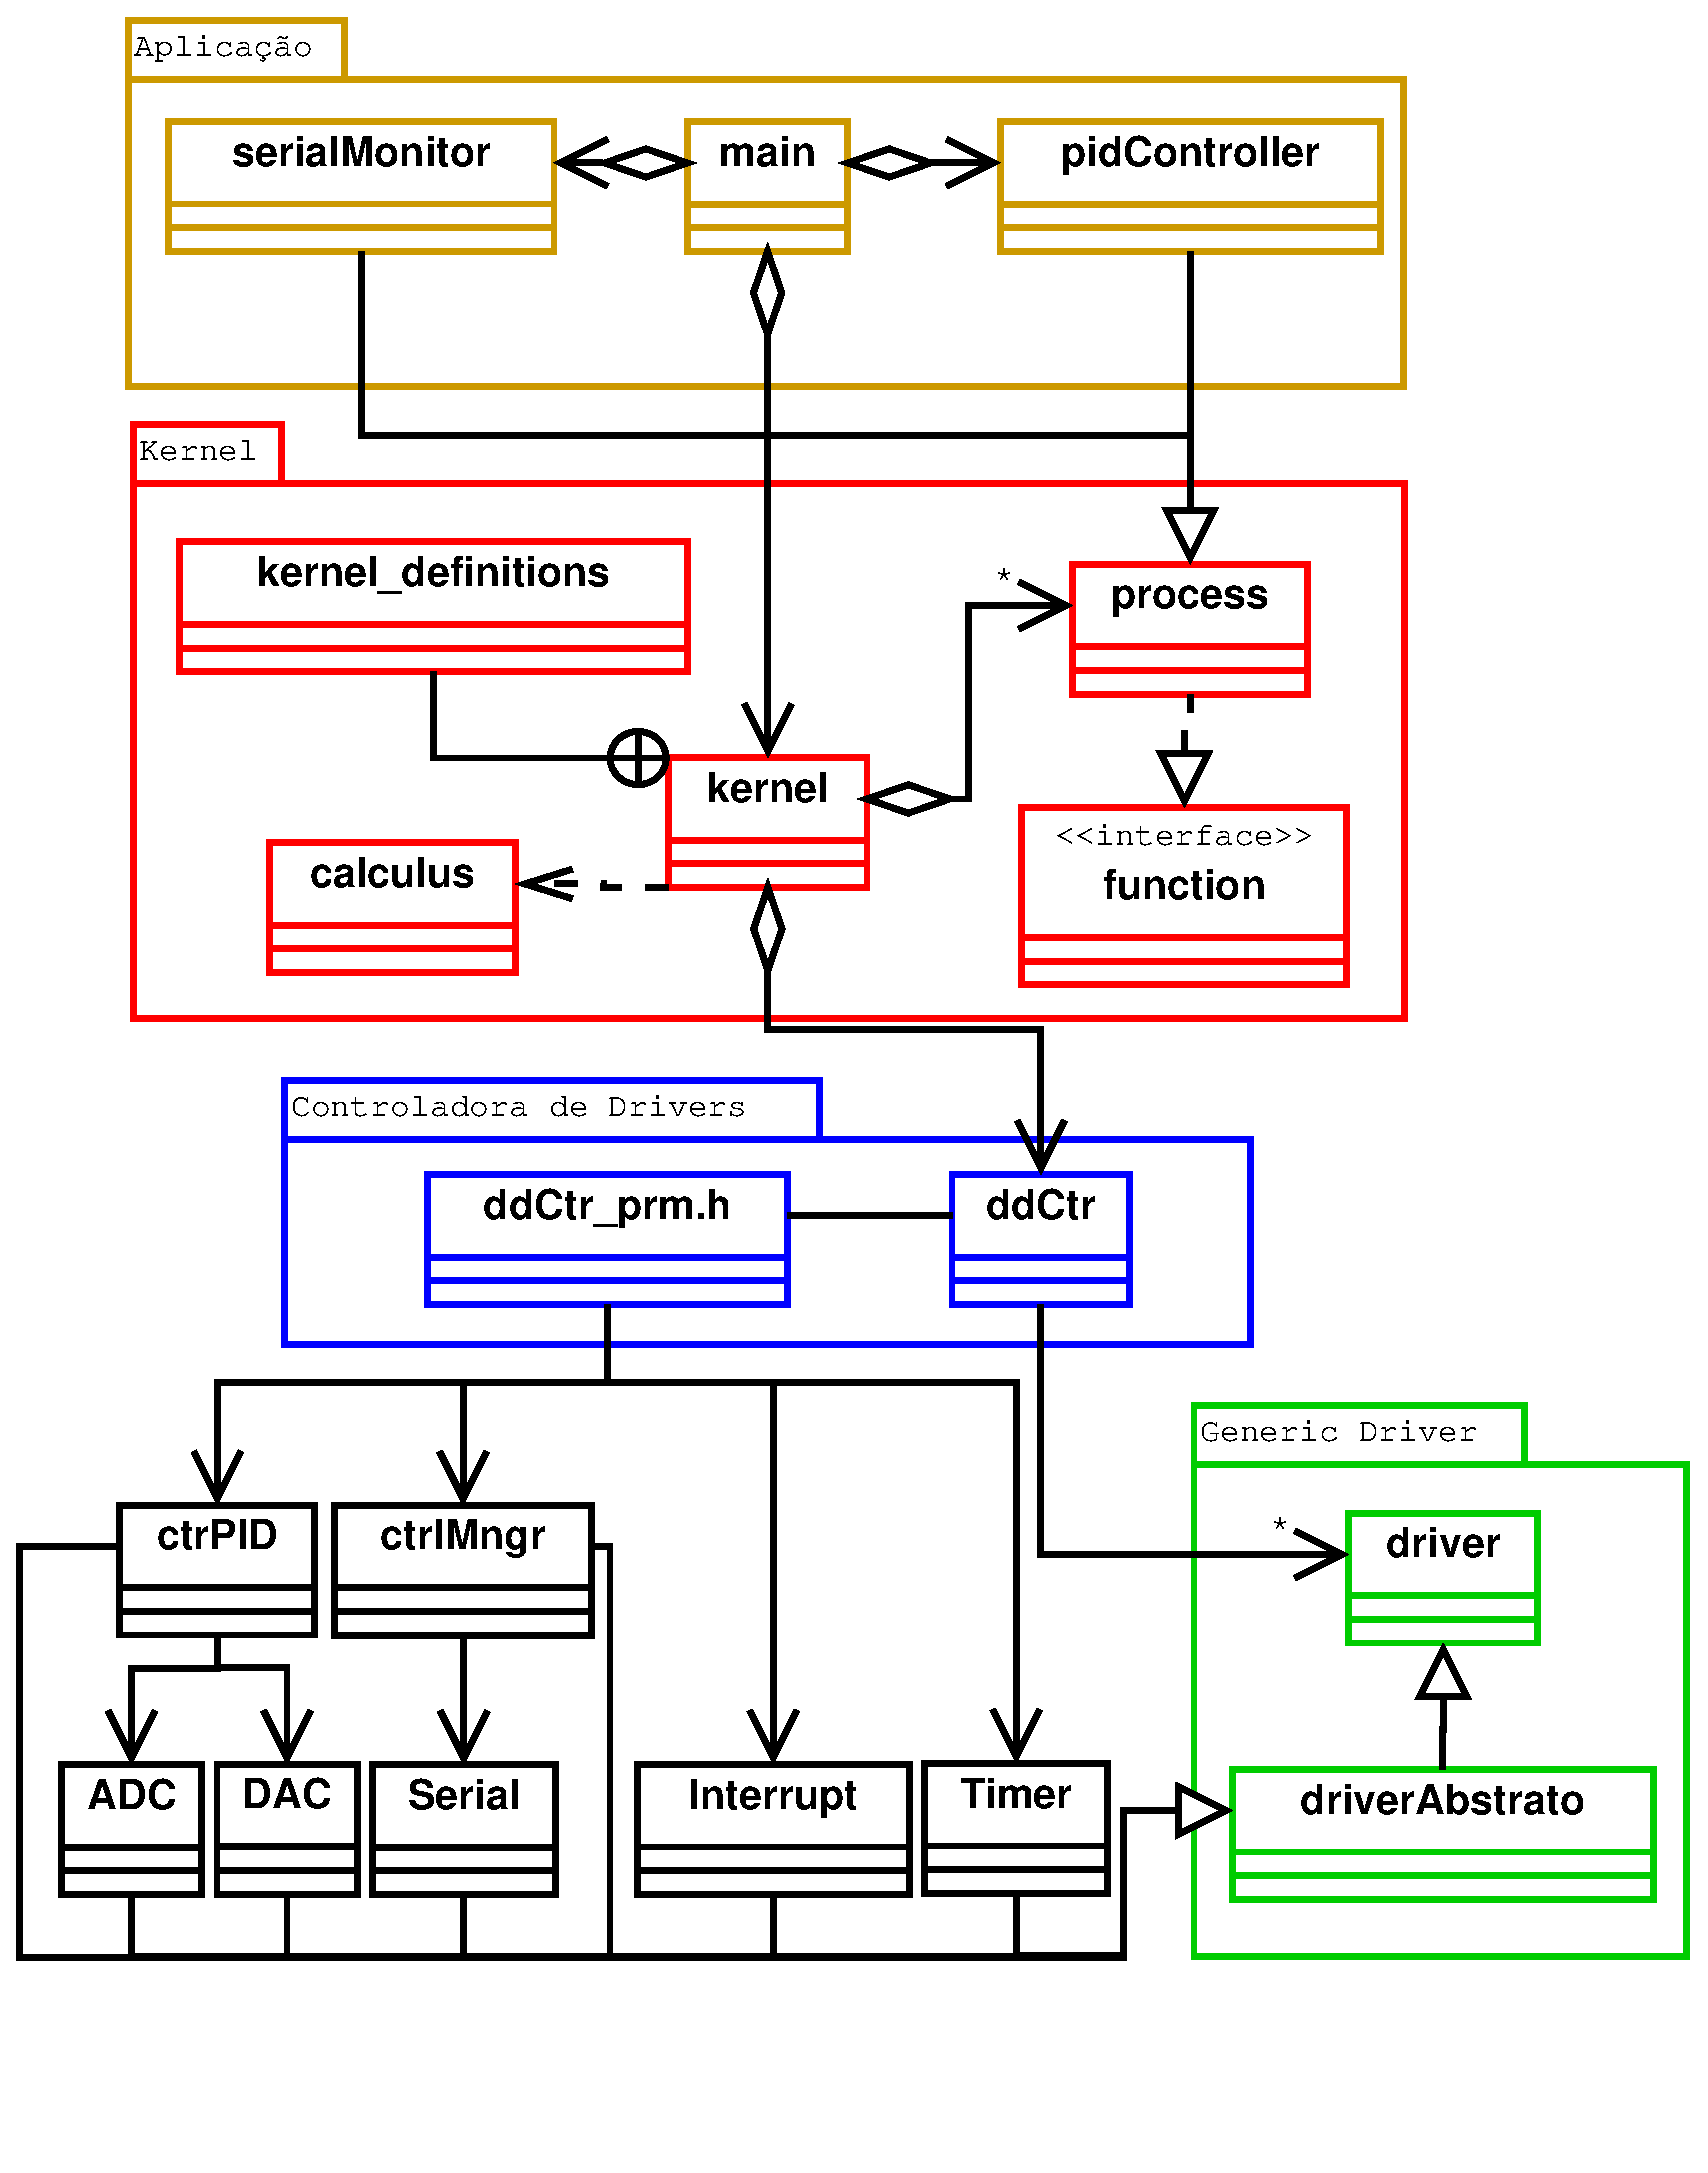
\includegraphics[width=13cm]{uml/umlCompleto.eps}
	\caption{Diagrama UML do sistema desenvolvido}
	\label{fig:diagramaClasse}
	\end{center}
\end{figure}

A aplicação pode ser composta de mais de um processo que são gerenciados pelo kernel através de uma estrutura do tipo \textit{process}. Estes processos são implementados como funções contendo \textit{loops} infinitos. A adição, remoção, pausa ou continuidade na execução dos processos é definida pelas interfaces disponibilizadas no kernel. Maiores detalhes do kernel e a implementação das rotinas são apresentados na próxima seção.

O desenvolvimento da controladora de \textit{drivers} pode ser visto no anexo~\ref{chap:controladora}. Desenvolveu-se uma interface bastante simples para gerenciamento das interações entre a aplicação e os dispositivos, sendo composta de apenas 3 funções. Esta simplificação foi possível pela utilização de uma estrutura comum para todos os drivers, apresentada em verde no diagrama da Figura~\ref{fig:diagramaClasse}.

Da estrutura apresentada, dois \textit{drivers} devem ser notados: \textit{drvPID} e \textit{ctrlMngr}. Embora gerenciados pela controladora como \textit{drivers} normais, eles não fazem acesso ao \textit{hardware} diretamente. Eles agrupam informações de outros \textit{drivers} ou provém novos modos de uso dos \textit{drivers} apresentados. 

O desenvolvimento se concentrou na implementação de uma troca de contexto segura em um \textit{microkernel}. A estrutura de \textit{microkernel} foi escolhida por questões de isolamento e segurança \cite{tanenbaum2006can}. Foi desenvolvida uma controladora de \textit{drivers} permitindo a exibição, armazenamento e análise dos dados recolhidos do sistema. Optou-se por um sistema de controle real, como plataforma de testes, principalmente por este tipo de sistema necessitar de execução em tempo real.

O Código~\ref{cod:kernelClock} apresenta a função responsável pela troca de contexto das tarefas e foi desenvolvido de acordo com as especificações apresentadas na Tabela~\ref{tab:StackSeguranca}.


\begin{lstlisting}[float,caption=Rotina responsável por executar a troca de contexto entre os processos,label=cod:kernelClock]
void interrupt kernelClock(void){
  //at this point CCR,D,X,Y,SP are stored on the stack
  volatile unsigned int SPdummy;     //stack pointer temporary value
  volatile unsigned int crc_on_stack;//point to the crc on the stack
  crc_on_stack = 1;           //just to avoid optmization error
    __asm PULD; __asm PULD;     //remove SPdummy & crc_on_stack
  __asm LDAA 0x30; __asm PSHA;//storing PPage on the stack
  __asm PSHD; __asm PSHD;     //recreating crc_on_stack & SPdummy
  __asm TSX;                  //fill SPdummy with actual stack position
  __asm STX SPdummy;
  
  //storing check value  
  if (pool[actualTask].Prio == RTOS){
    crc_on_stack  = hamming((unsigned char *)SPdummy+4,10);
  } else {
    crc_on_stack  = crc16((unsigned char *)SPdummy+4,10); 
  }
  __asm TSX;		  //save SP value on process info for further recover
  __asm STX SPdummy;
  pool[actualTask].StackPoint = SPdummy+2; //+2 to point to stack top
  if (pool[actualTask].Status == RUNNING){
    pool[actualTask].Status = READY;
  }
  actualTask = Scheduler();
  pool[actualTask].Status = RUNNING;
  SPdummy = pool[actualTask].StackPoint; 
  __asm LDX SPdummy; //load the next task SP from process info
  __asm TXS;
  __asm PSHD;        //restore space for SPdummy variable
  
  //reading check value and checking the data integrity
  if (pool[actualTask].Prio == RTOS){
    SPdummy  = hamming((unsigned char *)(pool[actualTask].StackPoint+2),10);
    if (crc_on_stack != SPdummy) { //making XOR to find bit changed
      crc_on_stack = (crc_on_stack^SPdummy) - 136; 
      if (crc_on_stack < 80){
*((unsigned char *) (pool[actualTask].StackPoint+2+(crc_on_stack/8))) = *((unsigned char *) (pool[actualTask].StackPoint+2+(crc_on_stack/8))) ^ (1<<(crc_on_stack%8));
      }
    }
  } else {
    SPdummy= crc16((unsigned char *)(pool[actualTask].StackPoint+2),10); 
    if (crc_on_stack != SPdummy) {
       SPdummy = restartTask(actualTask)-2;
       __asm LDX SPdummy;
       __asm TXS;
    }
  }
  __asm PULD; __asm PULD;     //remove crc_on_stack & SPdummy
  __asm PULA; __asm STAA 0x30;//set PPage for the next process
  CRGFLG = 0x80;              //clearing the RTI flag
  __asm RTI;                  //All other context loading is done by RTI
}
\end{lstlisting}

\chapter{Resultados}

Os testes foram realizados no kit de desenvolvimento Dragon12 com um processador de 8 \textit{bits}, com suporte a algumas operações de 16 \textit{bits}, e um \textit{clock} de 8 MHz. A placa é baseada no microcontrolador MC9S12DT256, com um conjunto de periféricos externos já embutidos. Entre os periféricos externos destaca-se o LTC1661 que é utilizado neste trabalho como saída analógica para o controlador implementado. %TODO ref

O sistema operacional foi desenvolvido tendo-se em mente a simplicidade de modo que a sobrecarga fosse mínima e a adaptação do código fácil. Uma primeira versão do sistema, portado para o processador PIC18f4550 é apresentada por \citeonline{de2013microkernel}. Após melhorias no sistema e a adição da preempção, esta versão foi portada para o processador HCS12. A comparação destas versões, bem como os dados de outros sistemas de tempo real, foram compilados na Tabela~\ref{tab:comOS}.

\begin{table}
\caption{Comparação de consumo de memória entre sistemas operacionais de tempo real}
\label{tab:comOS}
\begin{center}
	\begin{tabular}{|C{8.5cm}|C{3cm}|C{3cm}|}
		\hline
		Sistema Operacional & Consumo de Flash (mínimo) & Consumo de RAM (mínimo) \\
		\hline
		\hline
		VxWorks \cite{windRiver2013}       & $>$ 75.000 & - \\
		\hline
		FreeRTOS \cite{freertos2013online} & $>$ 6.000 & $>$ 800 \\
		\hline
		uC/OS \cite{micrium2013online}     & $>$ 5.000 & - \\
		\hline
		Microkernel \cite{de2013microkernel}   & 2.948 & 619 \\		
		\hline
		uOS \cite{vakulenko2011online}     & $>$ 2.000 & $>$ 200  \\
		\hline		
		BRTOS \cite{brtos2013online}       & $>$ 2.000 & $<$ 100  \\
		\hline
		Proposto (mínimo)    & 871 & 71 \\
		\hline		
		Proposto com algoritmo de correção sem \textit{lookup table}   & 1702 & 76 \\
			
		Proposto com algoritmo de correção com \textit{lookup table} na RAM    & 1729 & 620 \\
		\hline
		Proposto com algoritmo de correção com \textit{lookup table} na Flash    & 2273 & 76 \\
		\hline
	\end{tabular}
\end{center}
\end{table}

Os cinco bytes extras exigidos pelo sistema proposto com correção não se referem a consumo estático, mas às variáveis internas das funções que são alocadas na pilha. O grande aumento para o sistema proposto com as rotinas de correção otimizadas se deve, principalmente, ao uso de \textit{lookup-tables}, para o CRC de 512 bytes e para o Hamming de 32 bytes. Este consumo pode ser deslocado da RAM para a memória não volátil. Deste modo, o consumo de memória \textit{flash} passaria de 1729 para 2273, e o consumo de RAM volta ao patamar do sistema não otimizado, de 76 bytes.

Em termos de consumo de memória, o sistema proposto apresenta os menores valores entre os sistemas da Tabela~\ref{tab:comOS}. Mesmo quando considerada a versão com o sistema de correção ativo, os valores ainda são compatíveis com as alternativas. O gráfico na Figura~\ref{fig:consumoSO} apresenta em azul os valores base para o sistema operacional proposto com os dois escalonadores implementados. As barras em vermelho indicam o consumo de memória adicional para os três métodos de proteção deste trabalho (CRC, Hamming e Misto), além da controladora de dispositivos e do sistema de prioridade.


\section{Testes do controlador PID}
  
Este teste é focado na capacidade do sistema projetado de reproduzir corretamente as ações de controle mesmo sob falhas de memória e com excesso de processos para serem executados. O resultado do comportamento dinâmico destes testes não são significativos para este estudo, apenas a coerência destes resultados com as simulações é importante.

Durante os testes, o sistema de correção misto estava habilitado e erros na pilha de memória eram gerados a cada troca de contexto para estressar o sistema, tanto com o \textit{overhead} de processamento quanto com a possibilidade de falha para o sistema de controle.

A modelagem da planta (um circuito RC série) pode ser formulada a partir da relação entre tensão e corrente no capacitor. O detalhamento se encontra no anexo~\ref{chap:planta}. A equação a ser inserida no simulador, portanto, é:

\begin{equation}
	  \frac{V_{c}(s)}{V_{e}(s)} = \frac{1}{s + 1}
\end{equation}

Foi utilizado o \textit{software} \textit{Scilab 5.4.1} para validação dos resultados obtidos pelo sistema de controle. A Figura~\ref{sim_ma} apresenta o resultado da simulação da planta em malha aberta. A Figura~\ref{res_ma} apresenta as formas de onda obtidas no circuito real, gravadas pelo osciloscópio. 

\begin{figure}[ht]
        \center
        \begin{subfigure}[b]{0.55\textwidth}
        	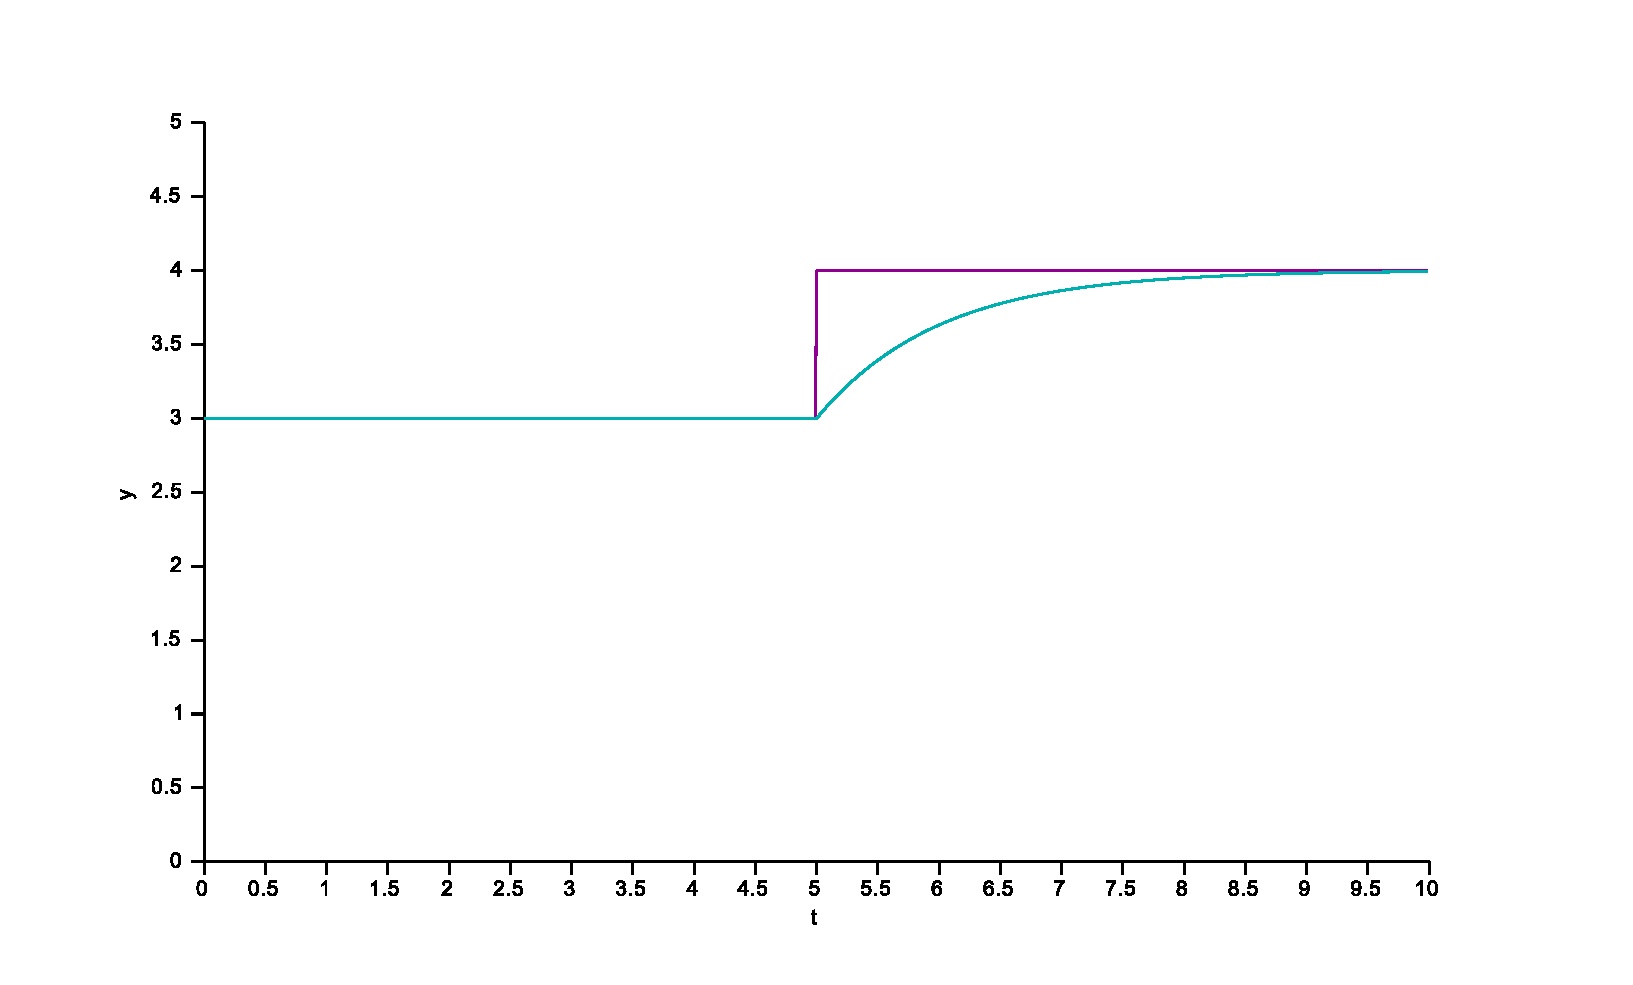
\includegraphics[width=\textwidth]{pid/openloop.pdf}
        	\caption{Simulação}
			\label{sim_ma}
        \end{subfigure}
        \begin{subfigure}[b]{0.4\textwidth}
        	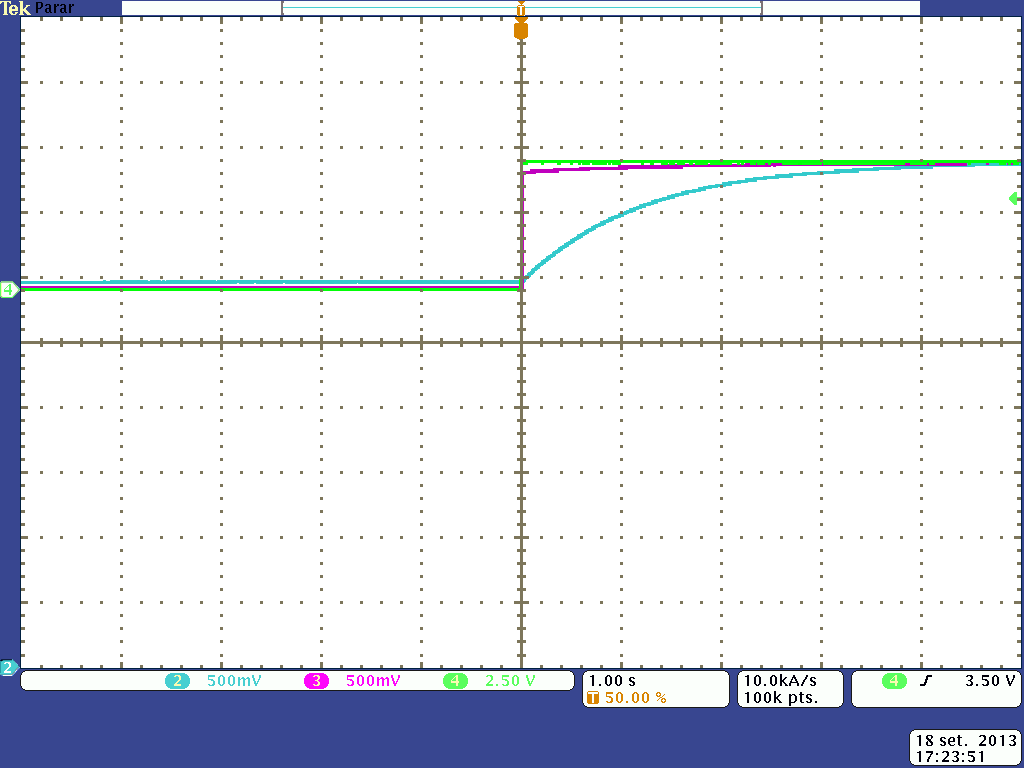
\includegraphics[width=\textwidth]{pid/openloop.png}
        	\caption{Teste}
        	\label{res_ma}
        \end{subfigure}
        \caption{Resposta do sistema ao degrau unitário em malha aberta}
\end{figure}

\chapter{Conclusão}

A utilização dos métodos de correção e detecção de erros, na proteção de regiões de memória críticas para a troca de contexto, funcionou conforme o esperado, evitando os erros e protegendo a continuidade da execução do sistema.

A proteção adicionada por estes métodos permite que um sistema microprocessado aumente sua confiabilidade frente a erros em \textit{bits} de memória ou falhas como \textit{stack overflow}. Mesmos nos testes de longa duração (120 horas), com erros sendo simulados a cada troca de contexto, com o sistema de detecção e correção habilitado, não houve problema observado.

Os testes realizados com o sistema de controle demonstraram que, na ausência de qualquer sistema de detecção ou correção, a troca do valor de um único bit pode paralisar todo o sistema. 

O consumo extra de memória, quando habilitado o sistema de correção e/ou detecção de erros, é pequeno, de 669 bytes, para memória não volátil (código) e de apenas 5 bytes, para memória volátil (RAM). Estes valores tornam a técnica implementável na maioria dos microcontroladores de baixo custo. A sobrecarga dos métodos otimizados se deve quase exclusivamente às tabelas, acrescendo um total de 544 bytes, de RAM ou de memória não volátil.

Quanto ao consumo de processamento, o algoritmo de detecção aumentou o tempo necessário para realizar uma troca de contexto. Quando observado o sistema original, sem nenhum tipo de correção ou detecção de erros, as trocas de contexto eram responsáveis por um consumo de 0,60\% do tempo de processamento disponível. A adição de um sistema de detecção de erros utilizando o algoritmo CCITT-CRC16 elevou este número para 12,65\%. Quando considerado o algoritmo de correção de erros de Hamming, o aumento é da ordem de 80 vezes, chegando a consumir quase metade do tempo disponível para processamento, 49,39\%. Estes valores, principalmente o último, poderiam inviabilizar o uso desta técnica em processadores de baixo custo, que apresentam também baixa capacidade de processamento.

Estes valores de consumo, no entanto, podem ser reduzidos em mais de 80\% com o uso de técnicas de otimização como \textit{lookup-tables}. Aplicando-se estas técnicas nos algoritmos utilizados, o sistema de correção por CRC passa a exigir apenas 1,46\% de processamento. No entanto a \textit{lookup-table} utilizada impacta no consumo de memória em cerca de 512 bytes.

Para o o algoritmo de Hamming, no entanto, o consumo de memória adicional é de apenas 16 bytes, mantendo mesmo assim uma redução da ordem de 80\%, atingindo o patamar de apenas 8,36\%. Isto viabiliza o uso destas técnicas em sistemas com poucos recursos computacionais. O algoritmo de Hamming otimizado se torna uma boa alternativa, pois apresentar um consumo menor que o algoritmo de CRC sem otimização sem gerar o gasto extra de memória do algoritmo de CRC otimizado.

A proposta de utilização de um modelo misto, de correção para processos de prioridade RT, e detecção para os demais processos, se mostrou muito interessante. Mantém-se um consumo próximo ao de um sistema com capacidade de detecção de erros (CRC) ao mesmo tempo que se garante a confiabilidade trazida pelo método de correção de erros (Hamming) para os processos mais críticos.

\citeonline{borchert2013generative} apresentam uma solução similar à desenvolvida neste trabalho. Eles fazem uso das mesmas técnicas de detecção e correção (CRC e Hamming) na proteção das estruturas de dados pertencentes às regiões críticas do \textit{kernel}. A abordagem utilizada, no entanto, é inviável para sistemas embarcados de baixo custo, visto que esta exige a utilização de uma linguagem orientada à objeto com capacidade de programação orientada à aspecto. A solução apresentada, fazendo uso apenas de recursos padronizados na linguagem C, permite a sua aplicabilidade em praticamente qualquer plataforma que tenha um compilador C.

Um ponto crítico em sistemas embarcados é a necessidade de tempo real para alguns processos. Segundo os testes realizados, não houve problemas em garantir o funcionamento do sistema de controle com o sistema de detecção e correção habilitados, mesmo simulando falhas na pilha a cada troca de contexto. Os resultados das ações de controle se mostraram iguais as simulações realizadas.

A questão de um invasor, no entanto, pode ser mais grave. Caso este possua conhecimento sobre o algoritmo utilizado no código de correção a abordagem do modo apresentado será ineficiente. Uma solução é a utilização um valor aleatório que possa ser atualizado automaticamente e utilizado como \textit{seed} na pilha de dados. Como as trocas de contexto acontecem em frequências relativamente altas, o sistema proposto, com a troca constante da \textit{seed}, inviabilizaria diversos tipos de ataques voltados à re-escrita da memória de pilha. 

As alternativas para a geração de códigos de checagem, que sejam de difícil quebra por parte do invasor, como algoritmos assimétricos, são caras do ponto de vista computacional. Deste modo, é possível que sua implementação em sistemas de baixo custo seja inviável, tornando a técnica apresentada como a única alternativa viável para este cenário.

\section{Trabalhos futuros}
Tendo em vista a tendência no aumento de dispositivos móveis e a preocupação com a redução de consumo, vislumbra-se a criação de rotinas ainda mais otimizadas para o cálculo dos bytes de correção e detecção dos erros. Isto permitiria que o sistema consumisse menos recursos computacionais e permanecesse mais tempo em modos de baixo consumo de energia.

Uma segunda frente de trabalho seria a adaptação do código para outras arquiteturas e/ou outros sistemas operacionais. O FreeRTOS é um dos candidatos naturais, pois tem todo seu código disponibilizado gratuitamente devido a licença GPL. Além disso, sua ampla utilização pode ser um bom ponto de disseminação da metodologia proposta.

Por fim a criação de um circuito dedicado que implemente a metodologia apresentada neste trabalho pode ser uma alternativa viável principalmente em sistemas baseados em FPGA e que façam uso de \textit{softcores}. A prototipagem de circuitos de hardware utilizando linguagens como VHDL é simples e retorna sistemas bastante otimizados principalmente no que tange as questões de velocidade. Isto aliado a alta capacidade de sintetizar lógicas combinacionais torna esta alternativa uma solução bastante interessante para implementar os algoritmos de detecção e correção de erros.

\section{Dificuldades}

O desenvolvimento da rotina de preempção foi um dos pontos críticos na implementação da metodologia. Esta rotina é executada por uma interrupção de hardware de modo que vários problemas se apresentam reunidos:
\begin{itemize}
\item a falta de acesso as variáveis não globais do sistema operacional;
\item uma pilha temporária devido ao salvamento dos registros da CPU, impedindo o acesso imediato à pilha do processo;
\item qualquer utilização de variáveis temporárias na rotina de interrupção insere dados extras na pilha atrapalhando sua manipulação;
\item a necessidade de baixo consumo, dado que este é um evento recorrente;
\item toda manipulação da pilha só pode ser feita em \textit{assembly}, e a integração desta com as linguagens de alto nível não é padronizada e altamente dependente do compilador e do \textit{hardware} utilizado. 
\end{itemize}

Estes fatores impactaram no desenvolvimento do projeto no tempo dispendido para o ajuste e desenvolvimento das rotinas de baixo nível.

A implementação do algoritmo de \textit{hamming} apresentou alguns problemas principalmente pela falta de recursos do processador em realizar operações bit à bit. A abordagem de utilizar apenas os bytes completos viabilizou o desenvolvimento para arquiteturas de baixo nível, no entanto uma comparação com o algoritmo original é interessante para definir os ganhos obtidos.

Para a realização dos testes, uma das primeiras dificuldades encontradas foi o modo de medição dos tempos gastos por cada porção da aplicação. A inserção de instrumentação no código se mostrou inviável pela carga adicional. Isto também faz com que a placa execute uma quantidade de código não necessária para a aplicação, podendo adulterar os resultados. A solução utilizada, de medição por valor médio, insere uma quantidade mínima de instruções apresentando um bom resultado.

A segunda dificuldade na realização dos testes foi o desenvolvimento de uma interface remota para controlar o número de processos em execução, criando-os e removendo-os com o sistema em funcionamento. Esta interface permite ainda a inserção de erros em bits da pilha de memória. A dificuldade se encontrou em desenvolver um protocolo que fosse simples e não influenciável pelos erros simulados na pilha. A utilização de um protocolo com capacidade de detecção de erros via CRC foi suficiente. 


\postextual

\bibliography{ref}

\apendices

\anexos

\chapter{Controladora}\label{chap:controladora}
A controladora foi projetada de modo que as requisições da aplicação ou do \textit{kernel} pudessem passar diretamente para os \textit{drivers} com o mínimo de \textit{overhead}. A estrutura básica da controladora desenvolvida pode ser vista na Figura~\ref{fig:ddctr}.

\begin{figure}[htbp]
	\begin{center}
	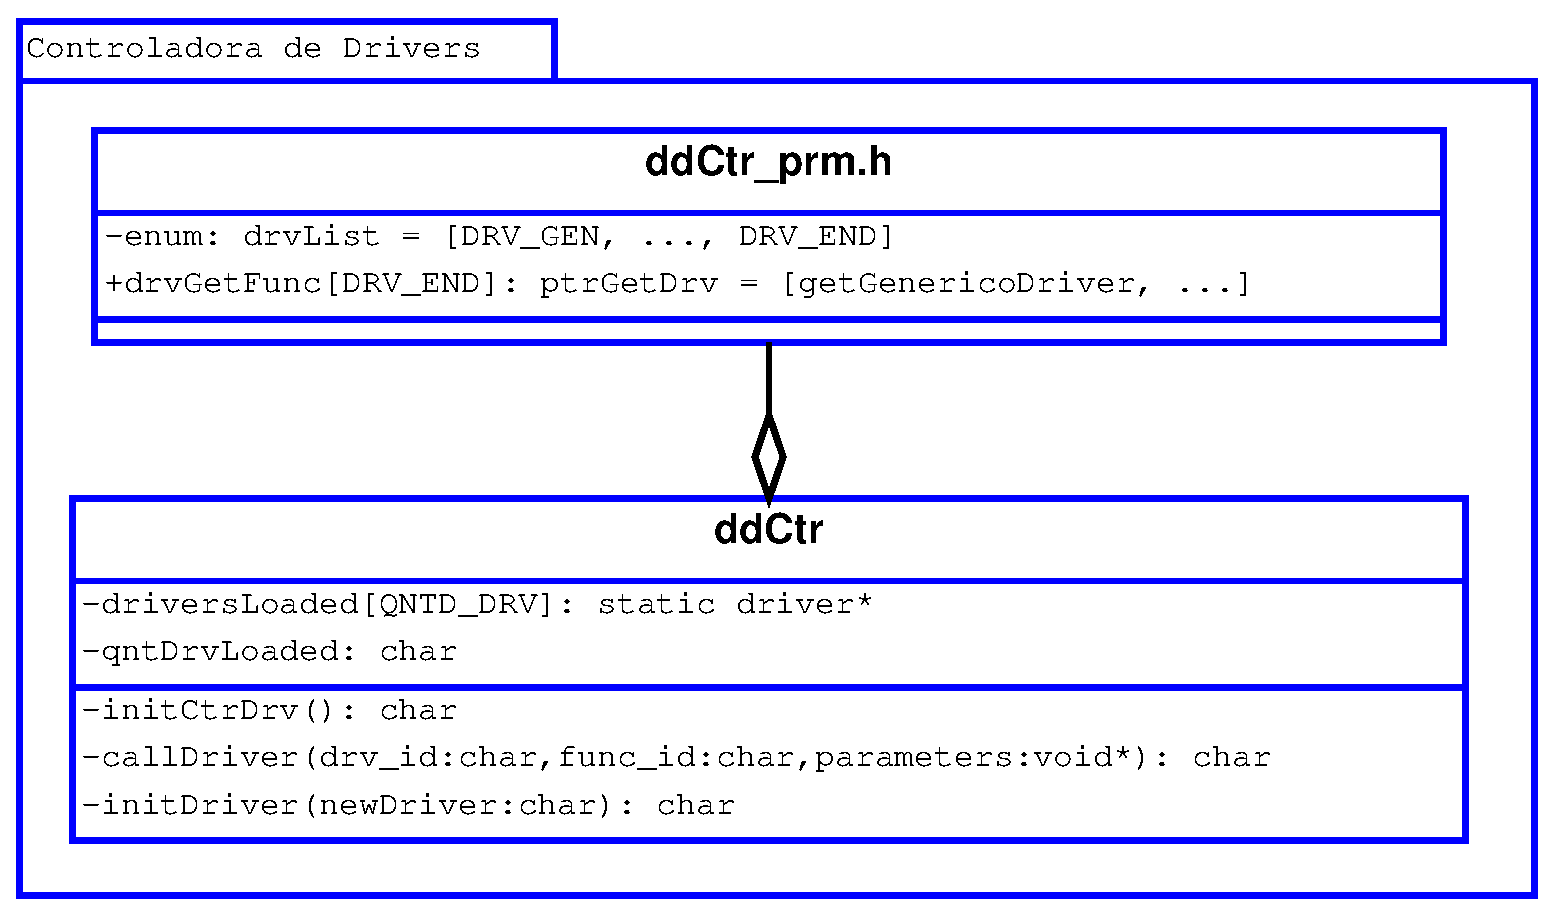
\includegraphics[width=12cm]{uml/umlControladora.eps}
	\caption{Diagrama da estrutura da controladora de \textit{drivers}}
	\label{fig:ddctr}
	\end{center}
\end{figure}

Para que a controladora opere sobre os \textit{drivers} é necessário obter um ponteiro para uma estrutura \textit{driver}. Isto é realizado por meio de uma função padronizada \textit{ptrGetDriver} implementada por cada \textit{driver} do sistema.

Esta função retorna uma \textit{struct} com todas as informações sobre o \textit{driver}. A posição na qual os ponteiros estão armazenados é definida por um enumerado, no arquivo \textit{ddCtr\_prm.h}, auxiliando na identificação do ponteiro para seu respectivo \textit{driver}. O código \ref{cod:driverDisponivel} exemplifica como realizar a ligação entre os \textit{drivers} e a controladora.

\begin{lstlisting}[float=h,caption=Definição dos \textit{drivers} disponíveis para uso,label=cod:driverDisponivel]
#include "drvInterrupt.h"
#include "drvTimer.h"
#include "drvLcd.h"
// enumerado para melhor acesso aos drivers
enum {
	DRV_INTERRUPT,
	DRV_TIMER,
	DRV_LCD,
	DRV_END
};
// funcoes de obtencao dos drivers
static ptrGetDrv drvInitVect[DRV_END] = {
	getInterruptDriver,
	getTimerDriver,
	getLCDDriver
};
\end{lstlisting}


\chapter{Equacionamento de um controlador digital do tipo PID}\label{chap:pid}

Sabe-se que a equação característica de um controlador PID é:

\begin{equation}
        G_{c}(s) = \frac{U(s)}{E(s)} = K_{p} + K_{d}.s + \frac{K_{i}}{s} 
\end{equation}

Para obter a sua forma digital é necessário utilizar a transformada~Z. A transformação bilinear é um modo de realizar essa conversão de modo simplificado. A transformada  é dada pela equação:

\begin{equation}
        s = \frac{2}{T} .\frac{z-1}{z+1}
\end{equation}

Aplicando a transformada na equação tem-se:

\begin{equation}
	\frac{U(z)}{E(z)} = \frac{k_{p}.2T(z+1)(z-1) + (2(z-1))^{2} . K_{d} + (T(z+1))^{2} . K_{i}}{T(z+1).2(z-1)} 
\end{equation}

\chapter{Protocolo de comunicação da aplicação teste}\label{chap:protocolo}

Para a comunicação entre a placa utilizada e o computador, foi criado um protocolo serial utilizando um CRC (\textit{Cyclic Redundancy Check}) de 16 \textit{bits} para evitar falhas de comunica\c{c}\~ao. \ A padronização seguiu os moldes do protocolo NMEA de comunicação GPS. Os pacotes foram definidos da seguinte forma:

\begin{center}
\textsf{{
{{\textless}START\_BYTE{\textgreater}{\textless}COMMAND\_BYTE{\textgreater}{\textless}PARAMETERS{\textgreater}{\textless}CRC\_16{\textgreater}{\textless}END\_BYTE{\textgreater}}
}}
\end{center}


\end{document}